\documentclass{../res/univ-projet}
\usepackage{graphicx}
\usepackage[francais]{babel}
\usepackage[T1]{fontenc}
\usepackage[utf8]{inputenc}
\usepackage{algorithmic}
\usepackage{algorithm}
\usepackage{dsfont}

\title{\'Etude du système d'OTP \og{}TOTP\fg{}}
\author{Les chats sauvages}

\projet{One Time Project}
\projdesc{\'Etude des systèmes de mots de passe jetable}
\filiere{M1SSI}
\logo{../res/logo_univ.png}

\begin{document}
\maketitle

\begin{abstract}
Ce document présente une analyse du système d'OTP \og{}TOTP\fg{}. Toutes les informations présentées et analysées proviennent de la RFC 6238 ainsi que de ses
correctifs. Le but de cet article est de déterminer dans quelle mesure le système TOTP est utilisable, sous quelles conditions et avec quelles garanties de sécurité.
Ce document sera mis en relation avec plusieurs autres afin de réaliser un comparatif entre les systèmes d'OTP majeurs.
\end{abstract}
\newpage
\tableofcontents
\newpage

\section{Pré-requis}
Le système d'authentification par mot de passe jetable \og{}TOTP\fg est une extension du système \og{}HOTP\fg{}, par conséquent, il repose sur les mêmes concepts. Ces 
derniers ayant déjà été donnés dans le document relatif à \og{}HOTP\fg{}, nous ne les détaillerons pas de nouveau ici.

\section{Généralités}
Le principe général de fonctionnement du système \og{}TOTP\fg{} est strictement identique à celui du système \og{}HOTP\fg{} à une différence près. Ici, un paramètre 
temporel est utilisé en lieu et place du compteur de synchronisation. Ainsi, la fonction $HMAC_K$ utilisée par \og{}HOTP\fg{} ne sera plus appelée avec pour paramètre la 
valeur du compteur de synchronisation mais avec la valeur $T = \lfloor{}\frac{curTime - T_0}{X}\rfloor{}$, où $curTime$ représente le temps Unix actuel, $T_0$ le temps Unix \og{}
d'origine\fg{} et $X$ un quantum de temps arbitraire.

\section{Approfondissement}
  \subsection{Génération et partage d'un secret}
    Le problème de génération et de partage de secret pour \og{}TOTP\fg{} est strictement identique à celui de \og{}HOTP\fg{} reportez vous au document relatif à ce 
    dernier pour un détails de méthodes.
    
  \subsection{Génération d'un mot de passe jetable}
    La génération des mots de passe jetables pour le système \og{}TOTP\fg{} est similaire à celle de \og{}HOTP\fg{} hormis sur le point du calcul de $HMAC$. En somme, la 
    génération peut être décrite par l'algorithme \ref{TOTP:gene}.
    \begin{algorithm}
      \caption{Génération d'un OTP par TOTP}
      \label{TOTP:gene}
   
      \begin{algorithmic}
	\REQUIRE $K$ une clef secrète
	\STATE $T \leftarrow \lfloor{}\frac{curTime - T_0}{X}\rfloor{}$
	\STATE $HVal \leftarrow HMAC(K, C)$
	\STATE $HVal \leftarrow tronc(HVal)$
	\STATE $HVal \leftarrow binToDec(HVal)$
	\newline
	\RETURN $HVal \bmod 10^L$ // L : longueur souhaitée de l'OTP
      \end{algorithmic}
    \end{algorithm}
    
    Les fonctions $tronc$ et $binToDec$ utilisées dans l'algorithme \ref{TOTP:gene} sont strictement identiques à celle utilisée dans l'algorithme de génération de 
    \og{}HOTP\fg{}. Référez vous au document traitant de \og{}HOTP\fg{} pour plus de détails.
    
  \subsection{Soumission et protocole de vérification}
    La vérification de mot de passe jetable suis le même schéma général que pour le système \og{}HOTP\fg{}. On trouve cependant quelque détails différents. Ces derniers 
    sont résumés dans l'algorithme \ref{TOTP:verif}.
    \begin{algorithm}
      \caption{Vérification d'un mot de passe jetable.}
      \label{TOTP:verif}
      
      \begin{algorithmic}
	\STATE $attentNB \leftarrow 0$
	\STATE $T \leftarrow \lfloor{}\frac{curTime - T_0 + \Delta_t}{X}\rfloor{}$
	\STATE $K \leftarrow$ clef secrète de l'utilisateur
	\STATE $OTP_1 \leftarrow TOTP_K(C)$
	\WHILE{$attentNB < MAX\_ATTENT$}
	  \STATE $OTP_2 \leftarrow$ récupérer\_OTP
	  \STATE $attentNB \leftarrow attentNB + 1$
	  \IF{$OTP_1 = OTP_2$}
	    \STATE accepter l'utilisateur
	  \ELSE
	    \IF{resynchro possible}
	      \STATE $resynchro$
	      \STATE accepter l'utilisateur
	    \ENDIF
	  \ENDIF
	\ENDWHILE
	\STATE $verouiller$
	\STATE $prevenir$
      \end{algorithmic}
    \end{algorithm}
    Ainsi, on retrouve bien le schéma général de vérification vu précédemment, utilisant la valeur $T$ décrite plus haut au lieu de celle du compteur de synchronisation.
    Cependant, dans cet algorithme, la valeur de $T$ est légèrement altérée afin d'y faire apparaitre la valeur $\Delta_t$. Cette dernière est utilisée pour garantir la 
    synchronisation temporelle entre le client et le serveur. Le fonctionnement et le calcul de cette valeur sont décrits dans la section \ref{OTP:syncSec}.
    
  \subsection{Synchronisation}
  \label{OTP:syncSec}
    De même que pour le système \og{}HOTP\fg{}, il est possible que le serveur et le client perdent leur synchronisation temporelle. Il suffit pour cela que
    l'horloge du client ou celle du serveur soit plus rapide que son homologue. Bien que l'utilisation de plus en plus répandue des serveur de synchronisation 
    temporelle mondiaux tende à réduire les possibilités de décalage des horloge, ce cas reste à envisager. C'est pourquoi on retrouve les fonction \og{}resynchro 
    possible\fg{} et $resynchro$, chargées d'assurer la cohérence des vérification d'OTP en cas de désynchronisation d'horloge. Les descriptions de ces fonctions sont 
    données dans les algorithme \ref{TOTP:isSynch} et \ref{TOTP:synch}.
    \begin{algorithm}
      \caption{Vérification de la possibilité de resynchronisation}
      \label{TOTP:isSynch}
      
      \begin{algorithmic}
	\REQUIRE $OTP$ la valeur de l'OTP fournie par l'utilisateur
	\REQUIRE $K$ la clef secrète de l'utilisation
	\STATE $T \leftarrow \lfloor{}\frac{curTime - T_0 + \Delta_t}{X}\rfloor{}$
	\STATE $MAX\_BWD \leftarrow b$ //$MAX\_BWD$ contient le nombre maximal de valeurs a vérifier vers l'arrière
	\STATE $MAX\_FWD \leftarrow a$ //$MAX\_FWD$ contient le nombre maximal de valeurs a vérifier vers l'avant
	\FOR{$i$ de $-MAX\_BWD$ à $MAX\_FWD$}
	  \STATE $OTP2 \leftarrow HOTP_K(T + i)$
	  \IF{$OTP = OTP2 AND not\_used(OTP)$}
	    \RETURN vrai
	  \ENDIF
	\ENDFOR
	\RETURN faux
      \end{algorithmic}
    \end{algorithm}
    
    \begin{algorithm}
      \caption{Resynchronisation}
      \label{TOTP:synch}
      
      \begin{algorithmic}
	\REQUIRE $OTP$ la valeur de l'OTP fournie par l'utilisateur
	\REQUIRE $K$ la clef secrète de l'utilisation
	\STATE $T \leftarrow \lfloor{}\frac{curTime - T_0 + \Delta_t}{X}\rfloor{}$
	\STATE $MAX\_BWD \leftarrow b$ //$MAX\_BWD$ contient le nombre maximal de valeurs a vérifier vers l'arrière
	\STATE $MAX\_FWD \leftarrow a$ //$MAX\_FWD$ contient le nombre maximal de valeurs a vérifier vers l'avant
	\FOR{$i$ de $-MAX\_BWD$ à $MAX\_FWD$}
	  \STATE $OTP2 \leftarrow HOTP_K(T + i)$
	  \IF{$OTP = OTP2 AND not\_used(OTP)$}
	    \STATE $\Delta_t \leftarrow \Delta_t + i * X$
	    \STATE accepter l'utilisateur
	  \ENDIF
	\ENDFOR
	\STATE rejeter l'utilisateur
      \end{algorithmic}
    \end{algorithm}
    
    Le fonctionnement de ces algorithmes est simple. Il s'agit de rechercher dans une fenêtre temporelle donnée une valeur d'OTP correspondant à celle donnée par 
    l'utilisateur. Si une telle valeur est trouvée, on calcule le décalage temporel entre les deux parties et on l'ajoute à la valeur courante du décalage $\Delta_t$.
    Sinon, l'utilisateur est rejeté.
    Comme pour le système \og{}HOTP\fg{}, ces deux fonctions pourront, en pratique, être fusionnées en une seule réalisant à la fois la vérification et la 
    synchronisation.
  
\section{Analyse générale et sécurité}
Analysons maintenant cette méthode et sa sécurité.

  \subsection{Avantages et intérêts}
  Le système \og{}TOTP\fg{} est une extension du système \og{}HOTP\fg{}. Par conséquent, il en reprend les principaux avantages. De plus, grâce à l'utilisation du temps 
  à la place d'un compteur de synchronisation, la synchronisation de ce système est plus difficile à perdre. En effet, lors de l'utilisation de \og{}HOTP\fg{}, il suffit 
  que l'utilisateur demande au \emph{token} plusieurs mots de passes de suite sans les utiliser pour perdre la synchronisation des parties. Pour \og{}TOTP\fg{}, le seul 
  moyen de perdre la synchronisation est que les horloges du client et du serveur n'avancent pas à la même vitesse. Hors, pour que la synchronisation soit décalée d'une 
  \og{}case\fg{}, il faut que le décalage d'horloge soit supérieur à $X$, qui , s'il est correctement choisi, doit être de l'ordre de quelques dizaines de seconde
  ce qui est considérable pour un décalage d'horloge. Bien entendu, il faut que les horloges du client et du serveur aient été synchronisées une première fois lors de 
  la première connexion ou lors de l'inscription de l'utilisateur sur le service.
  
  \subsection{Considérations de sécurité}
  La sécurité du protocole TOTP est directement héritée de celle de son parent HOTP. Ainsi, les probabilités de réussite des attaques exhaustives et les sensibilités au attaques 
  par collisions sont strictement identique modulo les valeurs choisies pour les tailles de fenêtre de resynchronisation et de nombre de tentatives autorisées.
  
    \subsubsection{Précautions et préconisation}
    En général, les précautions à prendre lors de l'utilisation de TOTP sont les mêmes que celles à prendre pour HOTP. Cependant, la taille de la fenêtre de resynchronisation
    doit être revue. En effet, lors de l'utilisation de TOTP, il est possible que le client soit décalé temporellement par rapport au serveur ou le contraire. De ce fait
    lors de la resynchronisation, le serveur doit confronter l'OTP non seulement avec les prochaines valeurs possibles mais aussi avec les précédentes. Aussi, pour éviter qu'un
    utilisateur puisse se connecter plusieurs fois avec le même mot de passe, il est nécessaire de conserver une liste des derniers OTP utilisés. Lors de la resynchronisation, 
    les valeurs de l'OTP données seront confrontées avec celles de la liste pour valider l'utilisation unique. La liste devra retenir au moins autant de mots de passes utilisés que 
    la taille de la fenêtre de resynchronisation vers l'arrière + 1.
    
    Au final, il sera raisonnable de fixer la taille de la fenêtre afin de permettre la validation à deux fenêtres vers l'arrière pour trois vers l'avant.
    
\section{Utilisations}
Tout comme HOTP, les utilisations pour l'implantation du protocole TOTP sont variées, on peut très bien s'en servir à des fins personnelles, pour sécuriser ses données ou 
dans un domaine professionnel.
  \subsection{Cas concrets d'utilisation}
  \begin{description}
   \item \textbf{Utilisation côté serveur}
   \begin{description}
    \item - Google avec son Google Autentificator
    \item - Amazon supporte également TOTP qui peut être utilisé avec les clients suivants: AWS (Multi-Factor Authentication) Amazon Virtual MFA ou le Google Authenticator.
    \item - DropBox
    \item - LastPass
    \item - GitHub
    \item - LinOTP
    \item - multiOTP
   \end{description}

   \item \textbf{Utilisation côté client}
   \begin{description}
    \item - Google Authenticator est un logiciel open-source qui est basé sur une authentification en deux étapes. Celui-ci est implémenté sur différentes plateformes 
	  mobiles comme iOS, Android, Blackberry, et il est aussi adaptable sur les modules PAM
	  \begin{figure}[h!]
	    \centerline{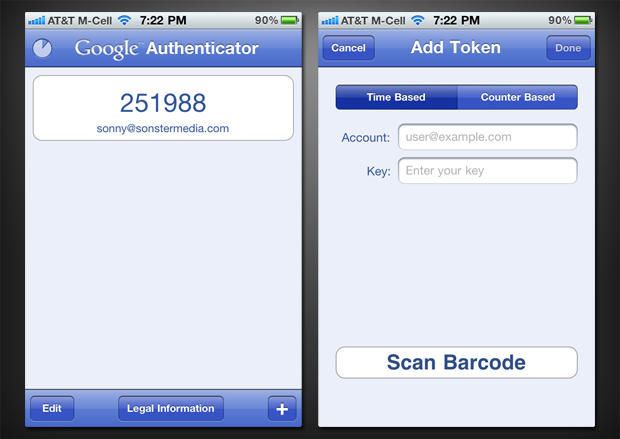
\includegraphics[scale=0.45]{imgHOTP/GoogleAuthenticator_2.jpg}}
	    \caption{Google Authenticator}
	  \end{figure}  
    \item - OATH Toolkit OATH Toolkit fournit une suite de composant pour la construction de systèmes d'authentification par mots de passe jetable. 
	  Les composant comprennent une librairie de programmation en C, un outil en lignes de commandes pour la génération et la validation d'OTP, et un PAM.
    \item - Microsoft's Authenticator est un logiciel pour les Windows Phone
    \item - Red Hat's FreeOT est un logiciel pour Android et iOS.
   \end{description}
  \end{description}
  
\section{Conclusion}
  \subsection{Pérénité du système}
   La pérennité du système TOTP est au moins aussi importante que celle de HOTP.
    
\end{document}
